% Mech Interp Dojo -- intro presentation (paper theme).
% Self-contained Beamer source. Build with (run twice for refs):
%   pdflatex mech_interp_dojo_intro_paper.tex
% Requires images in ./figures/ : mars-headshot.jpg, xor-geometry.png
\documentclass[aspectratio=169, 11pt, t]{beamer}
% Option 2: "Paper & Indigo" -- light, academic. Serif (Palatino).
\usepackage[T1]{fontenc}
\usepackage[utf8]{inputenc}
\usepackage{mathpazo}
\usefonttheme{serif}

\definecolor{mibg}{HTML}{FAF8F4}        % warm paper background (all content)
\definecolor{miink}{HTML}{1A1A2E}       % main text (near-black ink)
\definecolor{miaccent}{HTML}{3A0CA3}    % primary accent (indigo)
\definecolor{misharp}{HTML}{C75B39}     % sharp accent (burnt orange, darkened for contrast)
\definecolor{midark}{HTML}{2A0A6E}      % dark panel (indigo, title / closing)
\definecolor{midarktext}{HTML}{FAF8F4}  % text on dark
\definecolor{midarkaccent}{HTML}{CDB9FF}% accent on dark slides (light lavender)
\definecolor{mimuted}{HTML}{7A7686}     % muted captions / footers

% Shared structure for both color themes.
% Each theme file defines the colors (mibg, miink, miaccent, misharp, midark,
% midarktext, mimuted) and fonts, then \input's this file.

\usepackage{tikz}
\usetikzlibrary{positioning, arrows.meta, calc}
\usepackage[most]{tcolorbox}
\usepackage{amssymb}

\setbeamertemplate{navigation symbols}{}
\setbeamercolor{normal text}{fg=miink, bg=mibg}
\setbeamercolor{structure}{fg=miaccent}
\setbeamercolor{frametitle}{fg=miink}
\setbeamercolor{itemize item}{fg=miaccent}
\setbeamercolor{itemize subitem}{fg=miaccent}
\setbeamercolor{background canvas}{bg=mibg}
\setbeamerfont{frametitle}{series=\bfseries, size=\Large}
\setbeamerfont{framesubtitle}{size=\small}

% Frame title: bold, a little breathing room, no underline rule.
\setbeamertemplate{frametitle}{%
  \vspace*{0.7em}%
  {\usebeamerfont{frametitle}\usebeamercolor[fg]{frametitle}\insertframetitle\par}%
  \vspace*{0.2em}%
}

\setbeamertemplate{itemize item}{\small\raisebox{0.15ex}{\usebeamercolor[fg]{itemize item}\rule{0.7ex}{0.7ex}}}
\setbeamertemplate{itemize subitem}{\footnotesize{\usebeamercolor[fg]{itemize subitem}\textbullet}}

\newif\ifdarkslide \darkslidefalse
% subtle page number, bottom-right (theme/slide aware for contrast)
\setbeamertemplate{footline}{%
  \hfill{\ifdarkslide\color{midarktext!75}\else\color{miink!45}\fi\scriptsize\insertframenumber\,/\,\inserttotalframenumber}\hspace{3mm}\vspace{1.5mm}%
}

\hypersetup{colorlinks=true, urlcolor=miaccent, linkcolor=miaccent}

% ---- inline helpers ----
\newcommand{\acc}[1]{{\color{miaccent}#1}}          % accent on light slides
\newcommand{\dacc}[1]{{\color{midarkaccent}#1}}     % accent on dark slides
\newcommand{\pop}[1]{{\color{misharp}\textbf{#1}}}
\newcommand{\eyebrow}[1]{{\color{midarkaccent}\bfseries\footnotesize\MakeUppercase{#1}}}
\newcommand{\credit}[1]{{\color{mimuted}\scriptsize #1}}
\newcommand{\mono}[1]{{\ttfamily #1}}

% ---- dark slide color setup ----
% Use as: {\darkslide \begin{frame}[plain] ... \end{frame}}
% The enclosing braces scope the color changes to that one frame.
\newcommand{\darkslide}{%
  \darkslidetrue
  \setbeamercolor{background canvas}{bg=midark}%
  \setbeamercolor{normal text}{fg=midarktext, bg=midark}%
  \setbeamercolor{frametitle}{fg=midarktext}%
  \setbeamercolor{structure}{fg=midarkaccent}%
  \setbeamercolor{itemize item}{fg=midarkaccent}%
  \setbeamercolor{itemize subitem}{fg=midarkaccent}%
  \usebeamercolor[fg]{normal text}%
}

% ---- boxes ----
\newtcolorbox{callout}{
  enhanced, colback=miaccent!10!mibg, colframe=miaccent,
  boxrule=0.8pt, arc=3pt, left=8pt, right=8pt, top=6pt, bottom=6pt,
  halign=flush left,
}
\newtcolorbox{card}[1][]{
  enhanced, colback=mibg, colframe=miaccent!75!mibg,
  boxrule=0.8pt, arc=3pt, left=6pt, right=6pt, top=5pt, bottom=5pt,
  fonttitle=\bfseries\small, coltitle=miink,
  colbacktitle=miaccent!22!mibg, halign=flush left, #1
}
\newtcolorbox{codebox}{
  enhanced, colback=miink!4!mibg, colframe=miink!28!mibg,
  boxrule=0.7pt, arc=2pt, left=7pt, right=7pt, top=6pt, bottom=6pt,
  fontupper=\ttfamily\small,
}
% CTA banner: a bright card so it pops (and stays high contrast) on the dark closing slide.
\newtcolorbox{ctabox}{
  enhanced, colback=mibg, colframe=miaccent, coltext=miink,
  boxrule=1.3pt, arc=4pt, left=10pt, right=10pt, top=8pt, bottom=8pt,
  halign=center,
}

% ---- recurring motif: a faint 2x2 XOR checkerboard ----
\newcommand{\checkermotif}[2]{% #1 = side length, #2 = color
  \begin{tikzpicture}
    \fill[#2] (0,0) rectangle (#1,#1);
    \fill[#2] (#1,#1) rectangle (2*#1,2*#1);
  \end{tikzpicture}%
}

\begin{document}
% ===== Slide 1: Title (dark) =====
{\darkslide
\begin{frame}[plain]
  \begin{tikzpicture}[remember picture, overlay]
    \begin{scope}[shift={($(current page.north east)+(-2.1cm,-1.45cm)$)}]
      \fill[miaccent, opacity=0.16] (0,0) rectangle (0.7,0.7);
      \fill[miaccent, opacity=0.16] (0.7,0.7) rectangle (1.4,1.4);
      \draw[midarktext, opacity=0.18] (0,0) rectangle (1.4,1.4);
      \draw[midarktext, opacity=0.18] (0.7,0) -- (0.7,1.4);
      \draw[midarktext, opacity=0.18] (0,0.7) -- (1.4,0.7);
    \end{scope}
  \end{tikzpicture}
  \vspace*{0.7cm}
  {\eyebrow{Mech Interp Dojo}\par}
  \vspace{0.7cm}
  {\raggedright\color{midarktext}\huge\bfseries Understanding the expressivity of multi-headed attention\par}
  \vspace{0.9cm}

  {\raggedright\large\color{midarkaccent} Solving AI alignment by letting LLMs run wild on mech interp puzzles and formally verifying them. \par}
  \vfill
  {\color{mimuted}\small Intro meeting \textperiodcentered{} June 2026\par}
\end{frame}
}

% ===== About me (intro, light) =====
\begin{frame}{Hi, I'm Karthik}
  \large Physics PhD working on \acc{mechanistic interpretability} and \acc{AI alignment}.\normalsize\par
  \vspace{0.4cm}
  \begin{columns}[T]
    \begin{column}{0.55\textwidth}
      \begin{itemize}
        \item From \acc{IIT Madras} to a Physics PhD at the \acc{University of Amsterdam}.
        \item Recent alignment research: \pop{MATS 9.0} (Berkeley) and \pop{MARS 3.0} (Cambridge).
      \end{itemize}
      \vspace{0.6cm}
      \textbf{\acc{Find me}}\\[3pt]
      {\small
      \href{https://karthikviswanathn.github.io}{karthikviswanathn.github.io}\\[2pt]
      \href{https://scholar.google.com/citations?user=Qreb6HQAAAAJ}{Scholar} \textperiodcentered\ \href{https://github.com/karthikviswanathn}{GitHub} \textperiodcentered\ \href{https://linkedin.com/in/karthik-viswanathan}{LinkedIn}\\[2pt]
      vkarthik095@gmail.com\par}
    \end{column}
    \begin{column}{0.42\textwidth}
      \centering
      \begin{tikzpicture}
        \begin{scope}
          \clip[rounded corners=5pt] (0,0) rectangle (0.75\linewidth,0.75\linewidth);
          \node[anchor=south west, inner sep=0] at (0,0) {\includegraphics[width=0.75\linewidth]{figures/mars-headshot.jpg}};
        \end{scope}
        \draw[miaccent!60!mibg, line width=1pt, rounded corners=5pt] (0,0) rectangle (0.75\linewidth,0.75\linewidth);
      \end{tikzpicture}
    \end{column}
  \end{columns}
\end{frame}

% ===== Slide 2: What mechanistic interpretability is (light) =====
\begin{frame}{Mechanistic interpretability}
  \vspace{0.2cm}
  {\Large\itshape ``Reverse engineering neural networks, from the learned weights down to human-interpretable algorithms.''\par}
  \vspace{0.1cm}
  {\raggedleft\credit{-- a famous mechanistic interpretability researcher}\par}
  \vspace{0.55cm}
  \begin{itemize}
    \item The most fundamental level of the AI alignment problem. Knowing what a model computes inside is the basis for \acc{trusting and steering} it.
    \item Today this is mostly empirical. We rarely get \acc{exact, provable} statements about what a component can represent.
  \end{itemize}
  \vspace{0.35cm}
  \begin{callout}
    Our angle: start from the \pop{smallest questions we can answer exactly}.
  \end{callout}
\end{frame}

% ===== Slide 3: XOR in one attention layer (light) =====
\begin{frame}{A crisp instance: XOR in one attention layer}
  How many heads does a single attention layer need for \acc{XOR}? \pop{Exactly two.}
  \vspace{0.2cm}
  \begin{center}
    \begin{tcolorbox}[enhanced, width=0.74\textwidth, colback=white, colframe=miaccent!55!mibg,
      boxrule=0.6pt, arc=2pt, left=4pt, right=4pt, top=4pt, bottom=5pt, halign=center]
      
\includegraphics[width=\linewidth, height=3.8cm, keepaspectratio]{figures/xor-geometry.png}\\[4pt]
      {\itshape\small\color{miink!72} One attention head cannot compute XOR, but two can.\\
       Figure: ``How many attention heads do you need to do XOR?'', LessWrong.}
    \end{tcolorbox}
  \end{center}
\end{frame}

% ===== Slide 4: Scale up to H*(f) (light) =====
\begin{frame}{Scaling it up: from XOR to $H^{*}(f)$}
  \begin{callout}
    $H^{*}(f)$: the \pop{fewest attention heads} that compute a Boolean function $f:\{0,1\}^n\to\{0,1\}$, in a single attention layer with a linear readout.
  \end{callout}
  \vspace{0.15cm}
  \begin{columns}[c]
    \begin{column}{0.47\textwidth}
      \centering
      \resizebox{!}{3.7cm}{%
      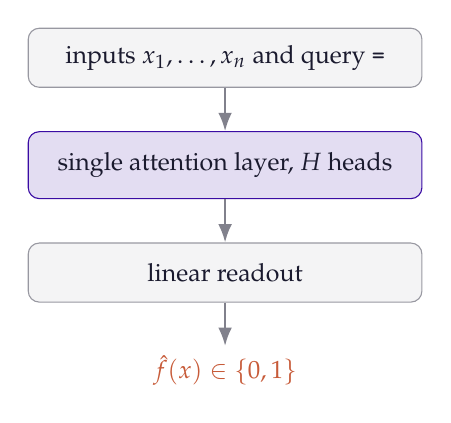
\begin{tikzpicture}[node distance=5.5mm, every node/.style={font=\small}]
        \node[draw=miink!45, fill=miink!5, rounded corners, minimum height=0.75cm, minimum width=5cm, text=miink] (tok) {inputs $x_1,\dots,x_n$ and query \texttt{=}};
        \node[draw=miaccent, fill=miaccent!14, rounded corners, minimum height=0.85cm, minimum width=5cm, below=of tok, text=miink] (att) {single attention layer, $H$ heads};
        \node[draw=miink!45, fill=miink!5, rounded corners, minimum height=0.75cm, minimum width=5cm, below=of att, text=miink] (read) {linear readout};
        \node[below=of read, text=misharp, font=\small\bfseries] (out) {$\hat{f}(x)\in\{0,1\}$};
        \draw[-{Latex}, miink!55, thick] (tok) -- (att);
        \draw[-{Latex}, miink!55, thick] (att) -- (read);
        \draw[-{Latex}, miink!55, thick] (read) -- (out);
      \end{tikzpicture}}
    \end{column}
    \begin{column}{0.5\textwidth}
      \begin{itemize}
        \item Proof of concept: $H^{*}(\mathrm{parity}_n)=n$, while $H^{*}(\mathrm{AND})=H^{*}(\mathrm{OR})=1$.
        \item A complexity measure \acc{native to transformers}.
      \end{itemize}
    \end{column}
  \end{columns}
\end{frame}

% ===== Slide 5: What we know so far (light) =====
\begin{frame}{What we know so far}
  \begin{columns}[T]
    \begin{column}{0.4\textwidth}
      \begin{card}[title=Lower bounds]
        $\deg_{\pm}(f)\leq H^{*}(f)$
      \end{card}
    \end{column}
    \begin{column}{0.4\textwidth}
      \begin{card}[title=Exact]
        $H^{*}(\mathrm{XOR}_n)=n$
      \end{card}
    \end{column}
  \end{columns}
  \vspace{0.4cm}
  {\centering
  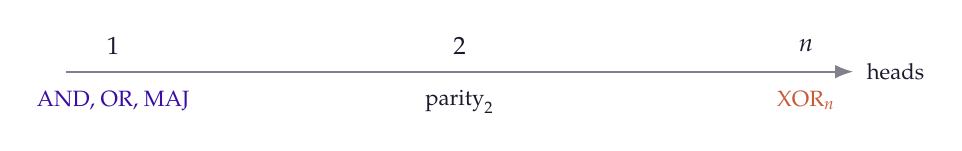
\begin{tikzpicture}
    \draw[-{Latex}, miink!55, thick] (0,0) -- (10,0);
    \node[text=miink, font=\small] at (0.6,0.33) {1};
    \node[text=miink, font=\small] at (5,0.33) {2};
    \node[text=miink, font=\small] at (9.4,0.33) {$n$};
    \node[below, text=miaccent, font=\footnotesize] at (0.6,-0.12) {AND, OR, MAJ};
    \node[below, text=miink, font=\footnotesize] at (5,-0.12) {$\mathrm{parity}_2$};
    \node[below, text=misharp, font=\footnotesize] at (9.4,-0.12) {$\mathrm{XOR}_n$};
    \node[right, text=miink, font=\footnotesize] at (10,0) {\,heads};
  \end{tikzpicture}\par}
  \vspace{0.2cm}
  {\centering\credit{We can bound many families, but no known invariant pins down $H^{*}(f)$ exactly. This is our first open problem.}\par}
\end{frame}

% ===== Slide 6: The grand goal (light) =====
\begin{frame}{The grand goal}
  \begin{columns}[T]
    \begin{column}{0.53\textwidth}
      \begin{itemize}
        \item Attention heads are \acc{one component}. The grand goal is to characterize \pop{each} transformer component, then chain them together.
        \item A compositional theory of \acc{what transformers can represent}.
        \item $H^{*}(f)$ is the \pop{first brick}.
      \end{itemize}
    \end{column}
    \begin{column}{0.45\textwidth}
      \centering
      \resizebox{0.99\linewidth}{!}{%
      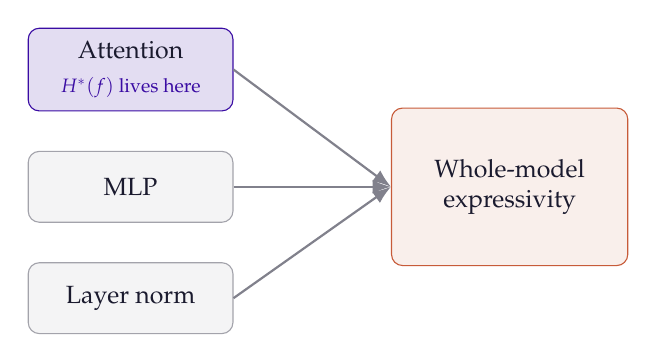
\begin{tikzpicture}[every node/.style={font=\small}, node distance=5mm]
        \node[draw=miaccent, fill=miaccent!14, rounded corners, minimum width=2.6cm, minimum height=1.05cm, align=center, text=miink] (att) {Attention\\[1pt]{\scriptsize\color{miaccent}$H^{*}(f)$ lives here}};
        \node[draw=miink!40, fill=miink!5, rounded corners, minimum width=2.6cm, minimum height=0.9cm, below=of att, text=miink] (mlp) {MLP};
        \node[draw=miink!40, fill=miink!5, rounded corners, minimum width=2.6cm, minimum height=0.9cm, below=of mlp, text=miink] (ln) {Layer norm};
        \node[right=2cm of mlp, draw=misharp, fill=misharp!10, rounded corners, minimum width=3cm, minimum height=2cm, align=center, text=miink] (all) {Whole-model\\expressivity};
        \draw[-{Latex}, miink!55, thick] (att.east) -- (all.west);
        \draw[-{Latex}, miink!55, thick] (mlp.east) -- (all.west);
        \draw[-{Latex}, miink!55, thick] (ln.east) -- (all.west);
      \end{tikzpicture}}
    \end{column}
  \end{columns}
\end{frame}

% ===== Slide 7: Why now (light) =====
\begin{frame}{Why now: LLMs change the economics of math}
  \begin{columns}[T]
    \begin{column}{0.49\textwidth}
      \begin{card}[title=LLMs can do real math, equal height group=whynow]
        GPT-5 produced solutions to open \href{https://openai.com/index/accelerating-science-gpt-5/}{Erd\H{o}s problems}, several later checked in Lean (2025).
      \end{card}
    \end{column}
    \begin{column}{0.49\textwidth}
      \begin{card}[title=LLMs can write Lean, equal height group=whynow]
        \href{https://www.galois.com/articles/claude-can-sometimes-prove-it}{Galois, \emph{``Claude Can (Sometimes) Prove It''}}: real proofs by \pop{directing a coding agent}, barely any hand written Lean.
      \end{card}
    \end{column}
  \end{columns}
  \vspace{0.45cm}
  \begin{callout}
    Proving results at this scale is finally \acc{within reach}.
  \end{callout}
\end{frame}

% ===== Slide 8: The dojo / Lean (light) =====
\begin{frame}{Trust, but verify: the Mech Interp Dojo}
  \begin{columns}[T]
    \begin{column}{0.55\textwidth}
      \begin{itemize}
        \item \acc{LLM drafts, Lean verifies.} LLM proofs hallucinate; \pop{Lean 4 + mathlib} checks every one and steers the proof generation.\textsuperscript{\textcolor{misharp}{\dag}}
        \item Humans ask the right questions and design abstractions; agents do the proof engineering.
      \end{itemize}
    \end{column}
    \begin{column}{0.44\textwidth}
      \begin{codebox}
        \textcolor{miaccent}{theorem} xor\_needs\_two :\\
        \hspace*{1.2em}Hstar (xor 2) = 2 := \textcolor{miaccent}{by}\\
        \hspace*{1.2em}\textcolor{mimuted}{-{}- formal proof}\\[5pt]
        {\color{green!55!black}$\checkmark$}~\textcolor{mimuted}{checked by Lean}
      \end{codebox}
    \end{column}
  \end{columns}
  \vfill
  {\footnotesize\color{mimuted}%
  \rule{0.32\linewidth}{0.3pt}\\[2pt]
  \textcolor{misharp}{\dag}~Even though this sounds like a neat plan, I have not yet seen verification help an LLM discover something it could not have found on its own. I am looking forward to seeing that happen here.\par}
\end{frame}

% ===== Slide 9: Deliverables (light) =====
\begin{frame}{Deliverables}
  \begin{columns}[T]
    \begin{column}{0.49\textwidth}
      \begin{card}[title=A library of lemmas, equal height group=deliv]
        Machine-checked theorems on \acc{what transformer components can and cannot represent}, from $H^{*}(f)$ and beyond. 
      \end{card}
    \end{column}
    \begin{column}{0.49\textwidth}
      \begin{card}[title=The Mech Interp Dojo, equal height group=deliv]
        An open source \pop{Lean 4 + mathlib} (modular) codebase that can be used by other researchers formally verifying proofs for mech interp.
      \end{card}
    \end{column}
  \end{columns}
\end{frame}

% ===== Slide 10: Where you come in (dark) + CTA =====
{\darkslide
\begin{frame}
  \frametitle{Where you come in}
  \centering
  {\small\color{midarktext!80} Three connected tracks, jump in anywhere.\par}
  \vspace{0.45cm}

  \resizebox{!}{4.9cm}{%
  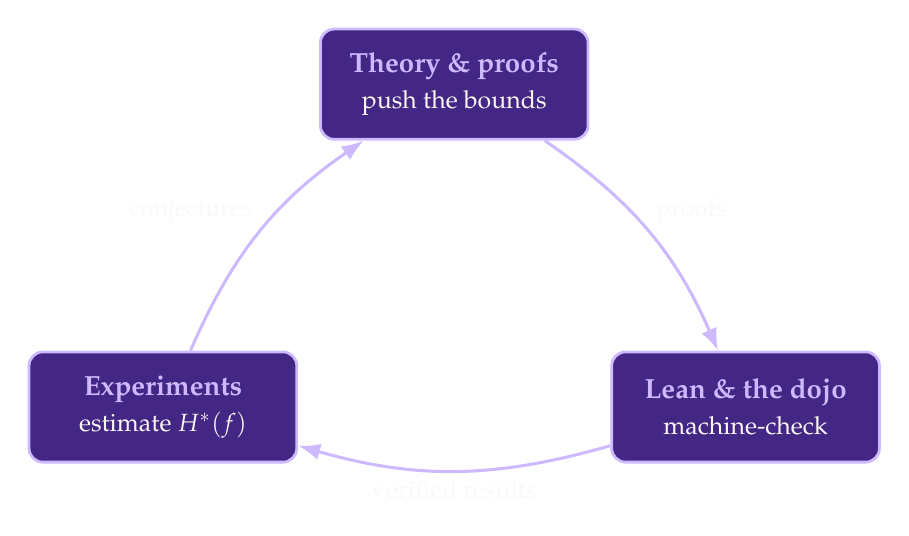
\begin{tikzpicture}[
    trk/.style={draw=midarkaccent, line width=1pt, rounded corners=5pt, fill=midarkaccent!16!midark,
                minimum width=3.4cm, minimum height=1.4cm, align=center, text=midarktext, inner sep=4pt},
    arr/.style={-{Latex}, midarkaccent, line width=1.1pt},
    lbl/.style={font=\small, text=midarktext!85, inner sep=3pt}]
    \node[trk] (theory) at (0,2.7) {\textbf{\dacc{Theory \& proofs}}\\[1pt]{\small push the bounds}};
    \node[trk] (exp) at (-3.7,-1.4) {\textbf{\dacc{Experiments}}\\[1pt]{\small estimate $H^{*}(f)$}};
    \node[trk] (lean) at (3.7,-1.4) {\textbf{\dacc{Lean \& the dojo}}\\[1pt]{\small machine-check}};
    \draw[arr] (exp) to[bend left=16] node[lbl, above left=-1pt]{conjectures} (theory);
    \draw[arr] (theory) to[bend left=16] node[lbl, above right=-1pt]{proofs} (lean);
    \draw[arr] (lean) to[bend left=16] node[lbl, below]{verified results} (exp);
  \end{tikzpicture}}
\end{frame}
}

% ===== Section divider: Logistics (dark) =====
{\darkslide
\begin{frame}[plain]
  \begin{tikzpicture}[remember picture, overlay]
    \begin{scope}[shift={($(current page.north east)+(-2.1cm,-1.45cm)$)}]
      \fill[miaccent, opacity=0.16] (0,0) rectangle (0.7,0.7);
      \fill[miaccent, opacity=0.16] (0.7,0.7) rectangle (1.4,1.4);
      \draw[midarktext, opacity=0.18] (0,0) rectangle (1.4,1.4);
      \draw[midarktext, opacity=0.18] (0.7,0) -- (0.7,1.4);
      \draw[midarktext, opacity=0.18] (0,0.7) -- (1.4,0.7);
    \end{scope}
  \end{tikzpicture}
  \vfill
  \centering
  {\Huge\bfseries\color{midarktext} Logistics}
  \vfill
\end{frame}
}

% ===== Slide 11: Important links (light) =====
\begin{frame}{Important links}
  \vspace{0.3cm}
  \begin{itemize}
    \item \textbf{Preliminary result:} \href{https://www.lesswrong.com/posts/T66BKwSufh5SfiPHm/how-many-attention-heads-do-you-need-to-do-xor-3}{How many attention heads do you need to do XOR?} (LessWrong)\vspace{0.3cm}
    \item \textbf{Project proposal:} \href{https://github.com/karthikviswanathn/how-many-attention-heads-xor/blob/main/proposal.pdf}{proposal.pdf}\vspace{0.3cm}
    \item \textbf{Code:} \href{https://github.com/karthikviswanathn/how-many-attention-heads-xor}{github.com/karthikviswanathn/how-many-attention-heads-xor}\vspace{0.3cm}
    \item \textbf{Team check-ins:} \href{https://docs.google.com/document/d/1h0ltuSWoPpPf_hGdqdma4re7ag9-dP8LKr7nP3rkYK4/edit?usp=sharing}{shared doc}\\[2pt]
      {\small\itshape Simplex-style check-ins: we follow the format from Simplex AI Safety (MATS).}
  \end{itemize}
\end{frame}

% ===== Slide 12: Some questions (light) =====
\begin{frame}{Some questions}
  \vspace{0.3cm}
  \begin{itemize}
    \item How should we communicate? \pop{Slack} or \pop{Discord}?\vspace{0.35cm}
    \item How often should we meet?\vspace{0.35cm}
    \item LLM credits: should we apply to \href{https://bluedot.org/programs/rapid-grants}{Rapid Grants} (BlueDot Impact)?
  \end{itemize}
\end{frame}

% ===== Slide 13: Thank you (dark) =====
{\darkslide
\begin{frame}[plain]
  \begin{tikzpicture}[remember picture, overlay]
    \begin{scope}[shift={($(current page.north east)+(-2.1cm,-1.45cm)$)}]
      \fill[miaccent, opacity=0.16] (0,0) rectangle (0.7,0.7);
      \fill[miaccent, opacity=0.16] (0.7,0.7) rectangle (1.4,1.4);
      \draw[midarktext, opacity=0.18] (0,0) rectangle (1.4,1.4);
      \draw[midarktext, opacity=0.18] (0.7,0) -- (0.7,1.4);
      \draw[midarktext, opacity=0.18] (0,0.7) -- (1.4,0.7);
    \end{scope}
  \end{tikzpicture}
  \vfill
  \centering
  {\Huge\bfseries\color{midarktext} Thank you!}\\[0.6cm]
  {\large\dacc{Let's solve AI alignment, one verified proof at a time!}}
  \vfill
\end{frame}
}
\end{document}
